%!TEX program = xelatex
% 完整编译: xelatex -> bibtex -> xelatex -> xelatex
\documentclass[lang=cn,11pt,a4paper,cite=numbers]{elegantpaper}
\title{基于布隆过滤器的Redis缓存穿透解决方案}
% 作者与单位
\author{xxx  xxxxxx}
% \institute{xxxxx}

% 版本号
% \version{0.9}
\version{}
% 日期
% \date{\zhtoday}
\date{}

% 本文档命令
\usepackage{array}
\newcommand{\ccr}[1]{\makecell{{\color{#1}\rule{1cm}{1cm}}}}





\begin{document}

\maketitle

\begin{abstract}本文论述了redis作为缓存数据库的优势与使用场景,剖析了在使用Redis作为缓存服务器时所存在的一个缓存穿透的问题,讨论了两种缓存穿透解决方案及其优劣势,然后对布隆过滤器的原理进行了解析,最终使用布隆过滤器整合Redis和数据库进行缓存穿透的实验的设计,得出了使用布隆过滤器能极大的提升服务器查询性能的结论,缓解Redis缓存数据库和磁盘数据库的压力,避免服务器因为缓存穿透这个漏洞而让黑客有机可乘,影响正常的业务。最后,对本文进行总结并探讨了布隆过滤器存在的缺陷以及更多的解决方案。
\keywords{布隆过滤器,Redis,缓存穿透}
\end{abstract}

\section{Redis概述}
\subsection{什么是Redis}
\paragraph{}Redis是一个高性能的NoSQL数据库,它是一个基于键值对的缓存与存储系统,遵守BSD协议并且完全开源。Redis通过设置各种键值数据类型来适应不同场景下的缓存与存储需求。同时Redis的诸多高层级功能使其可以胜任消息队列,任务队列等不同角色。
\subsection{将Redis引入应用和数据库之间的好处}
\begin{figure}[!htb]
    \centering
    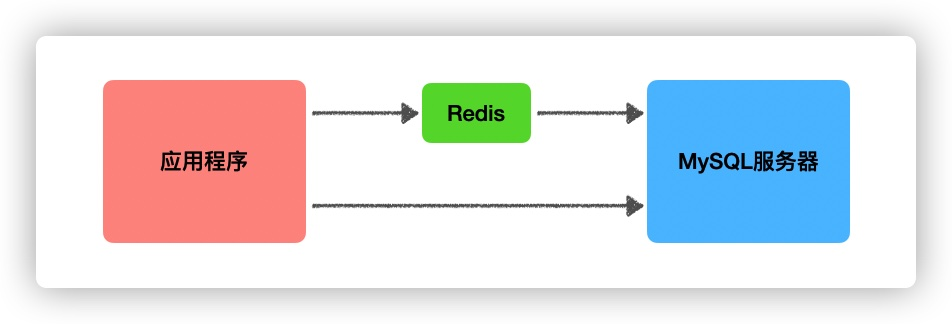
\includegraphics[width=0.7\textwidth]{1.jpg}
    \caption{将Redis引入应用和数据库之间}
\end{figure}
\paragraph{}使用Redis,最主要的功能就是它的缓存,就如计算机的高速缓存,当我们要访问某些数据时,先去Redis中找,看其是否存在,若不存在,则再访问数据库,同时将数据存入Redis,下次访问的时候就可以直接从Redis中读取,在一个小项目中,你可能感觉不到性能的提升,但是若同时有几十万,上百万的访问量时,其对性能的提升是飞跃的,极大地减小了数据库的压力,提升了数据查询的速度。
\subsection{Redis优势}
Redis运行在内存中但是可以持久化到磁盘,所以在对不同数据集进行高速读写时需要权衡内存,因为数据量不能大于硬件内存。在内存数据库方面的另一个优点是,相比在磁盘上相同的复杂的数据结构,在内存中操作起来非常简单,这样Redis可以做很多内部复杂性很强的事情。同时,在磁盘格式方面他们是紧凑的以追加的方式产生的,因为他们并不需要进行随机访问。

Redis有着更为复杂的数据结构并且提供对他们的原子性操作,Redis支持二进制案例的 Strings, Lists, Hashes, Sets 及 Ordered Sets 数据类型操作。Redis的数据类型都是基于基本数据结构的同时对程序员透明,无需进行额外的抽象。

同时,Redis还有很多丰富的特性,Redis可以为每个键设置生存时间,生存时间到后期会自动删除,这一功能可以利用Redis作为缓存系统来调用。除此之外, Redis的列表类型键可以用来实现队列,并且支持阻塞式读取,可以容易地实现一个高性能的优先级队列,同时在更高层上,Redis还支持"发布/订阅"的消息模式,可以基于此构建聊天室。

\section{缓存穿透原理剖析}
\paragraph{}缓存穿透是指查询一个一定不存在的数据,由于缓存不命中,并且出于容错考虑, 如果从存储层查不到数据则不写入缓存,这将导致这个不存在的数据每次请求都要到存储层去查询,失去了缓存的意义。以下我们通过图解来解析一下发生缓存穿透的原理:
\begin{enumerate}[label=\arabic*).]
    \item \textit{情况一:缓存存在}\\
    情况一是正常情况,应用访问服务器,命中缓存,缓存直接返回数据,避免了进行数据库的查询。
    \begin{figure}[!htb]
        \centering
        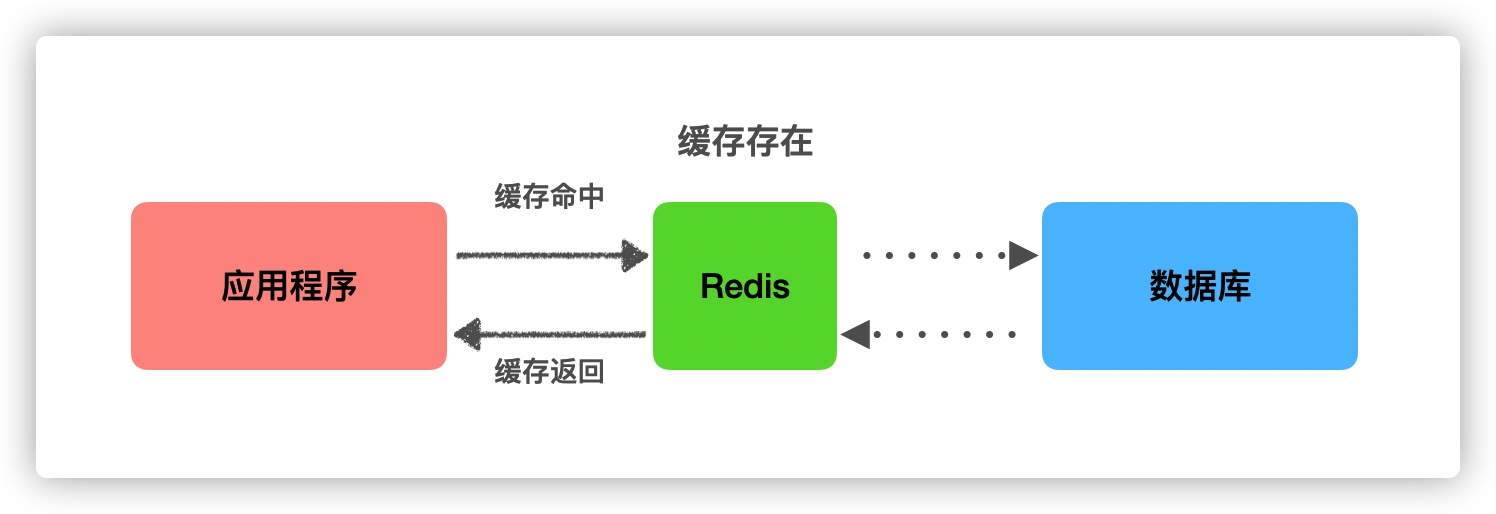
\includegraphics[width=0.7\textwidth]{2.jpg}
        \caption{缓存存在情况}
    \end{figure}
    \item \textit{情况二:缓存不存在,数据库存在}\\
    情况二也是正常情况,应用访问服务器,没有命中缓存,此时服务查询数据库中的数据,查到数据存在,把数据写入缓存,并返回数据给应用。一般发生这种情况的原因有两种:
    \begin{figure}[!htb]
        \centering
        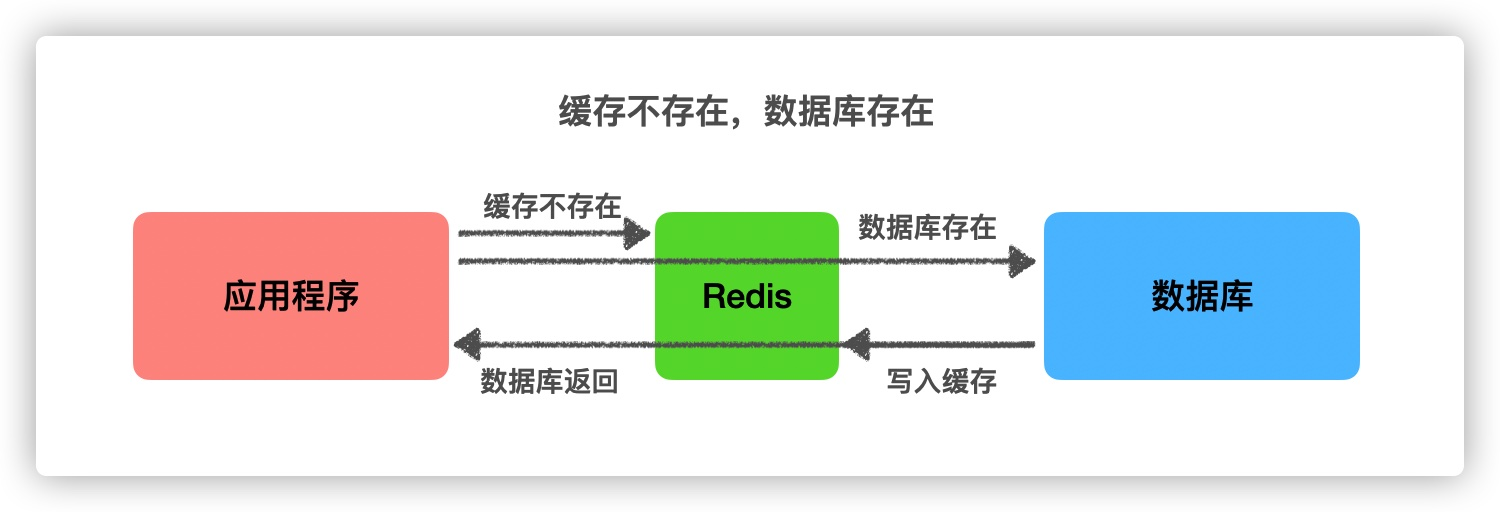
\includegraphics[width=0.7\textwidth]{3.jpg}
        \caption{缓存不存在,数据库存在}
    \end{figure}
    \begin{enumerate}
        \item 数据库刚刚更新,还没来得及加载进缓存
        \item Redis缓存的expire时间过期了
    \end{enumerate}

    \item \textit{情况三:缓存不存在,数据库不存在}\\
    如果应用每一次去数据库中查询不存在的值,且这个值每一次都不一样,Redis在这个过程中失去了屏障的作用了,被叫做缓存穿透。
    \begin{figure}[!htb]
        \centering
        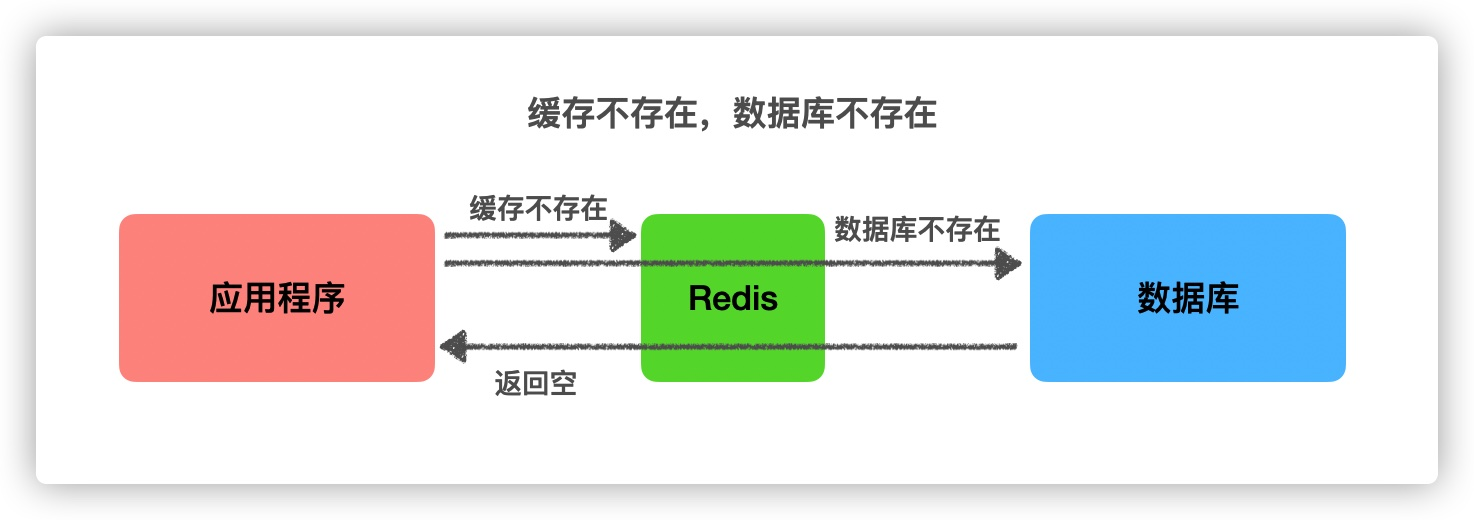
\includegraphics[width=0.7\textwidth]{4.jpg}
        \caption{缓存不存在,数据库不存在}
    \end{figure}
    如果发生缓存穿透,则对底层数据源压力过大,如果我们的底层数据源不具备高并发性,就有可能被会击溃我们的服务器。比如一个黑客故意制造我们缓存中不存在的key发送大量的请求,就会导致请求直接落到数据库上。
  \end{enumerate}


\section{缓存穿透的解决方案}
\paragraph{}解决缓存穿透的大致思路有两个:一个是缓存空对象,另一个是使用布隆过滤器。
\subsection{缓存空对象}
\begin{figure}[!htb]
    \centering
    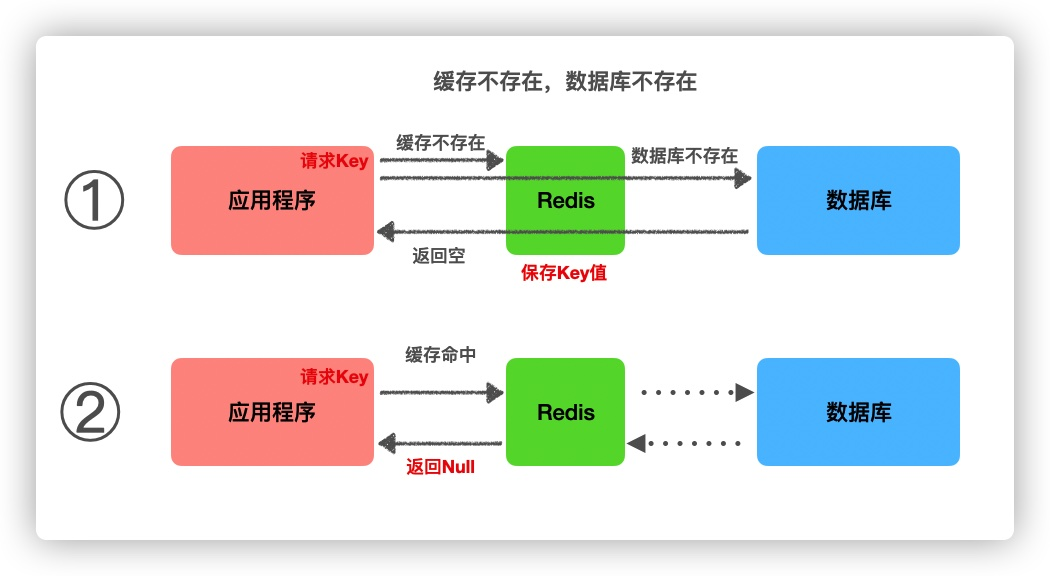
\includegraphics[width=0.7\textwidth]{5.jpg}
    \caption{缓存空对象}
\end{figure}
\paragraph{}定义:如上图所示,当缓存查询不到之后,仍然将空对象保留到Redis中(可能是保留几分钟或者一段时间,具体问题具体分析),下次新的请求(同一个key)将会从Redis中获取到数据,从而保护了后端的数据库。适用一些数据命中不高,数据频繁变化实时性高的一些业务。代码的维护成本低,但是有如下两个问题:
\begin{enumerate}
    \item 第一是空值做了缓存,意味着缓存系统中存了更多的key-value,也就是需要更多空间(虽然空值少,但是耐不住海量访问),解决方法是我们可以设置一个较短的过期时间。
    \item 第二是数据会有一段时间窗口的不一致,假如,Cache设置了5分钟过期,此时Storage确实有了这个数据的值,那此段时间就会出现数据不一致,解决方法是我们可以利用消息或者其他方式,清除掉Cache中的数据。
  \end{enumerate}
\subsection{布隆过滤器}
\begin{figure}[!htb]
    \centering
    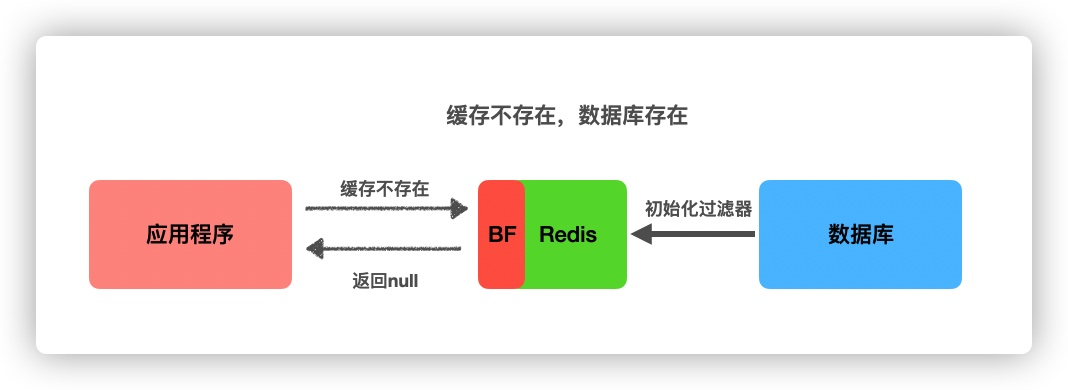
\includegraphics[width=0.7\textwidth]{6.jpg}
    \caption{布隆过滤器}
\end{figure}
\paragraph{}如上图所示,在访问所有资源之前,将存在的key用布隆过滤器提前保存起来,做第一层拦截,如果经过布隆过滤器,数据不存在,则不用访问数据库,Redis缓存层直接返回null。适用于数据命中不高,数据相对固定实时性低,通常是数据集较大的情况。
\subsection{两种方法对比}
\begin{table}[!htb]
    \centering
    \caption{缓存空对象和布隆过滤器对比图}
      \begin{tabular}{*{3}{>{\scriptsize}c}}
      \hline
      \textbf{解决缓存穿透} & \textbf{适用场景} & \textbf{维护成本}\\
      \hline
      缓存空对象  & 数据命中不高;数据频繁变化实时性高 & 需要过多的缓存空间;数据不一致\\
      布隆过滤器  & 数据命中不高;数据相对固定实时性低 & 代码维护相对复杂;缓存空间占用少\\
      \hline
      \end{tabular}%
    \label{tab:donation}%
  \end{table}%
\paragraph{}可以看出,使用布隆过滤器对于缓存空间的占用极小,我们知道我们的内存空间都是有效的,在使用小内存空间的情况下,就能解决缓存穿透的问题,且可以防止由于缓存空对象所带来的数据不一致的问题。

\section{布隆过滤器原理解析}
\subsection{哈希函数}
\paragraph{}哈希函数的概念是:将任意大小的数据转换成特定大小的数据的函数,转换后的数据称为哈希值或哈希编码。如下是一幅示意图:\\
\begin{figure}[!htb]
    \centering
    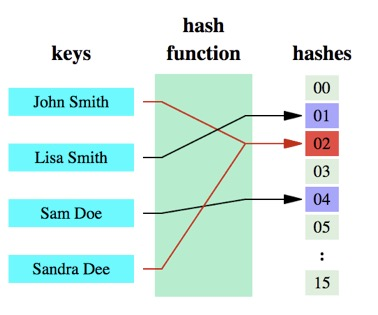
\includegraphics[width=0.7\textwidth]{7.jpg}
    \caption{哈希函数}
\end{figure}
\paragraph{}可以明显的看到,原始数据经过哈希函数的映射后称为了一个个的哈希编码,数据得到压缩。哈希函数是实现哈希表和布隆过滤器的基础。
\subsection{布隆过滤器}
\paragraph{}布隆过滤器(Bloom Filter)的核心实现是一个超大的位数组和几个哈希函数。假设位数组的长度为m,哈希函数的个数为k。
\begin{figure}[!htb]
    \centering
    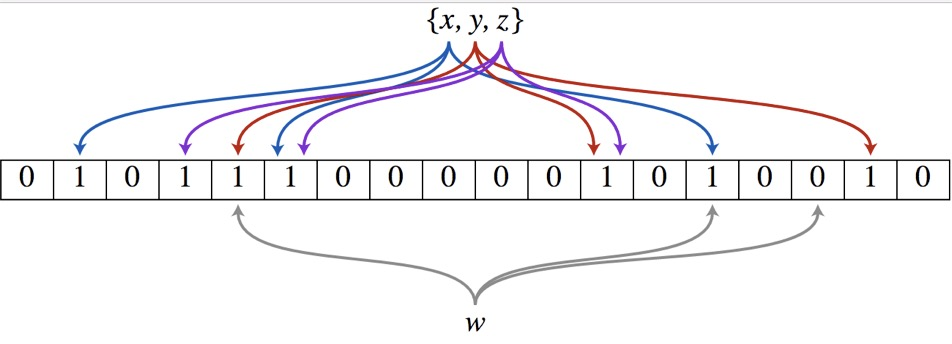
\includegraphics[width=0.7\textwidth]{8.jpg}
    \caption{布隆过滤器原理}
\end{figure}
\paragraph{}具体的操作流程:假设集合里面有3个元素{x, y, z},哈希函数的个数为3。首先将位数组进行初始化,将里面每个位都设置位0。对于集合里面的每一个元素,将元素依次通过3个哈希函数进行映射,每次映射都会产生一个哈希值,这个值对应位数组上面的一个点,然后将位数组对应的位置标记为1。查询W元素是否存在集合中的时候,同样的方法将W通过哈希映射到位数组上的3个点。如果3个点的其中有一个点不为1,则可以判断该元素一定不存在集合中。反之,如果3个点都为1,则该元素可能存在集合中。注意:此处不能判断该元素是否一定存在集合中,可能存在一定的误判率。可以从图中可以看到:假设某个元素通过映射对应下标为4,5,6这3个点。虽然这3个点都为1,但是很明显这3个点是不同元素经过哈希得到的位置,因此这种情况说明元素虽然不在集合中,也可能对应的都是1,这是误判率存在的原因。
\paragraph{布隆过滤器添加元素}
\begin{enumerate}
    \item 将要添加的元素给k个哈希函数
    \item 得到对应于位数组上的k个位置
    \item 将这k个位置设为1
\end{enumerate}
\paragraph{布隆过滤器查询元素}
\begin{enumerate}
    \item 将要查询的元素给k个哈希函数
    \item 得到对应于位数组上的k个位置
    \item 如果k个位置有一个为0,则肯定不在集合中
    \item 如果k个位置全部为1,则可能在集合中
\end{enumerate}
\paragraph{}总结来说,如果布隆过滤器判断元素在集合中存在,则元素不一定存在;如果布隆过滤器判断元素在集合中不存在,则元素一定不存在;如果元素实际存在,布隆过滤器一定判断存在;如果元素实际不存在,布隆过滤器可能判断存在.

\section{Redis整合布隆过滤器}
\subsection{环境依赖}
\begin{enumerate}[label=\arabic*).]
    \item \textit{布隆过滤器}\\
    我们使用google的Guava中编写好的BloomFilter,如图所示。
    \begin{figure}[!htb]
        \centering
        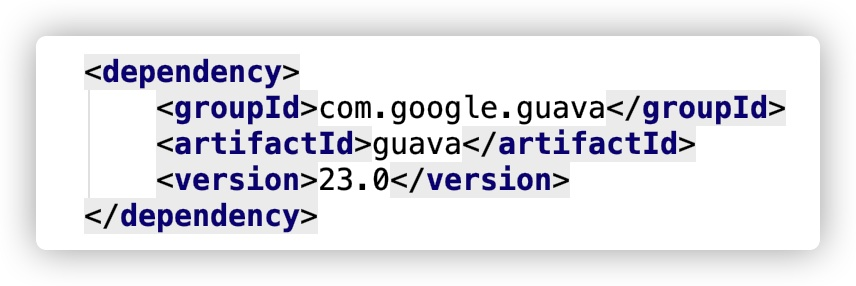
\includegraphics[width=0.7\textwidth]{9_1.jpg}
        \caption{布隆过滤器Maven导入}
    \end{figure}
        
    \item \textit{Redis \& Jedis}\\
    Redis 5.0.3 (00000000/0) 64 bit\\
    jedis 2.8.0
    \item \textit{其他环境依赖}\\
    JUnit、Druid连接池、mysql驱动
  \end{enumerate}
\subsection{实验设计}

\paragraph{}本次设计了一个用户(User)数据库作为底层数据源,数据库的字段如下:
\begin{figure}[!htb]
    \centering
    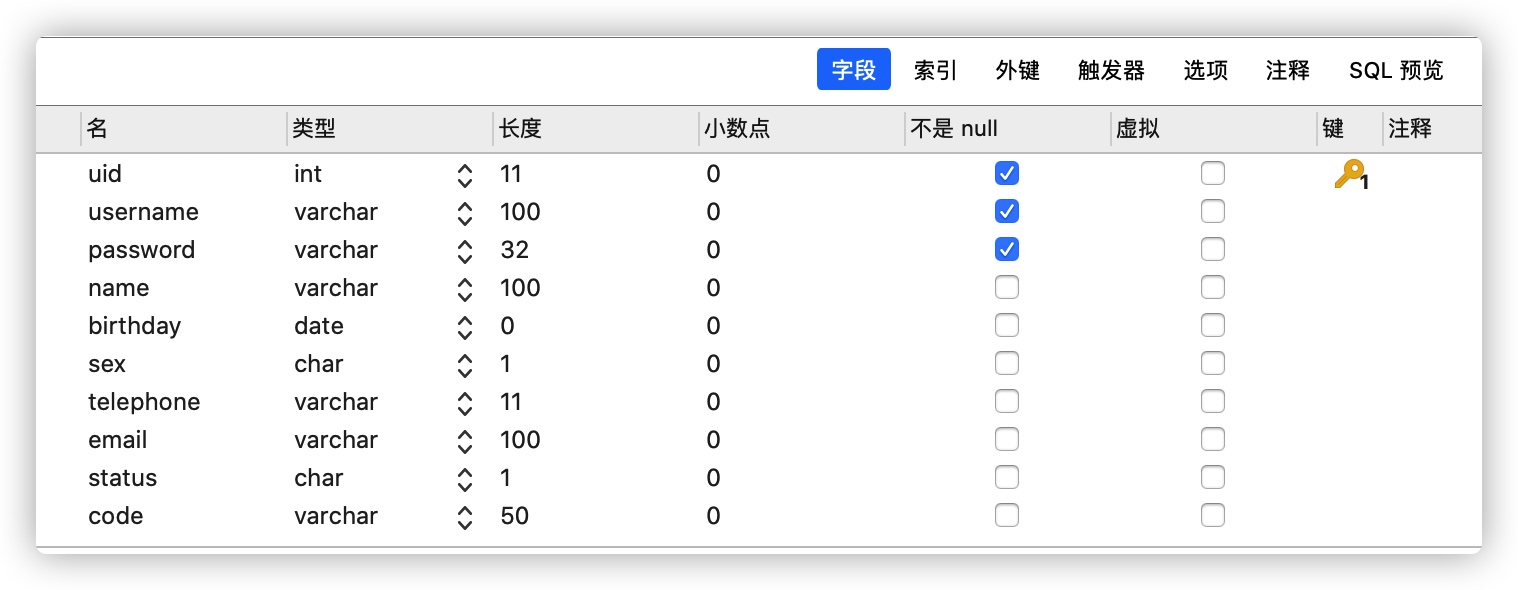
\includegraphics[width=0.7\textwidth]{9_3.jpg}
    \caption{数据表}
\end{figure}

\paragraph{}使用数据库连接池调用数据库,读取全部数据信息。
\begin{figure}[!htb]
    \centering
    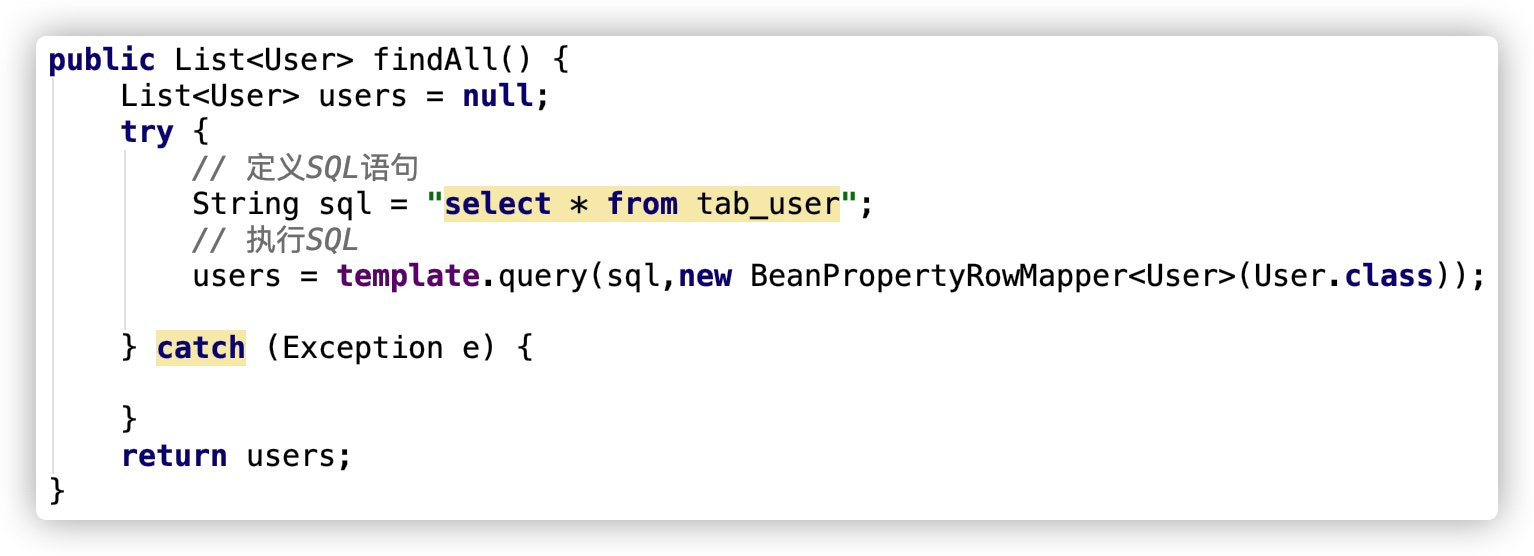
\includegraphics[width=0.7\textwidth]{9_5.jpg}
    \caption{使用数据库连接池}
\end{figure}

\paragraph{}初始化阶段,从数据库中读取全部的User数据信息,使用序列化工具序列化数据并将数据加载进Redis缓存中。
\begin{figure}[!htb]
    \centering
    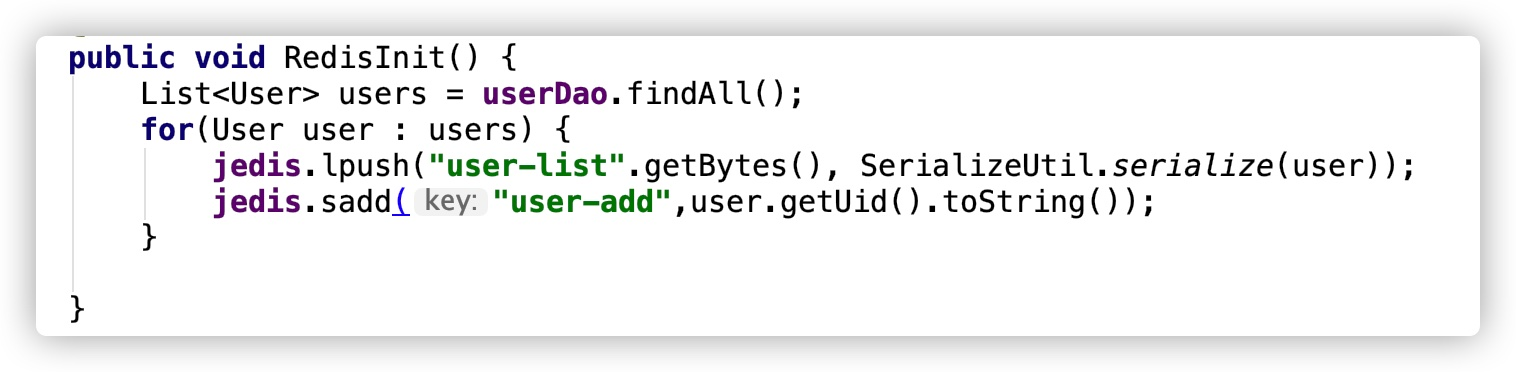
\includegraphics[width=0.7\textwidth]{9_4.jpg}
    \caption{初始化Redis缓存}
\end{figure}

\paragraph{}初始化布隆过滤器,从数据库中读取User数据信息,并将User信息的uid加载进布隆过滤器当中,这里我们设定布隆过滤器的exceptedInsertion大小为10000,其所占用的空间约为1KB,可以看出布隆过滤器所占用的空间非常的小。
\begin{figure}[!htb]
    \centering
    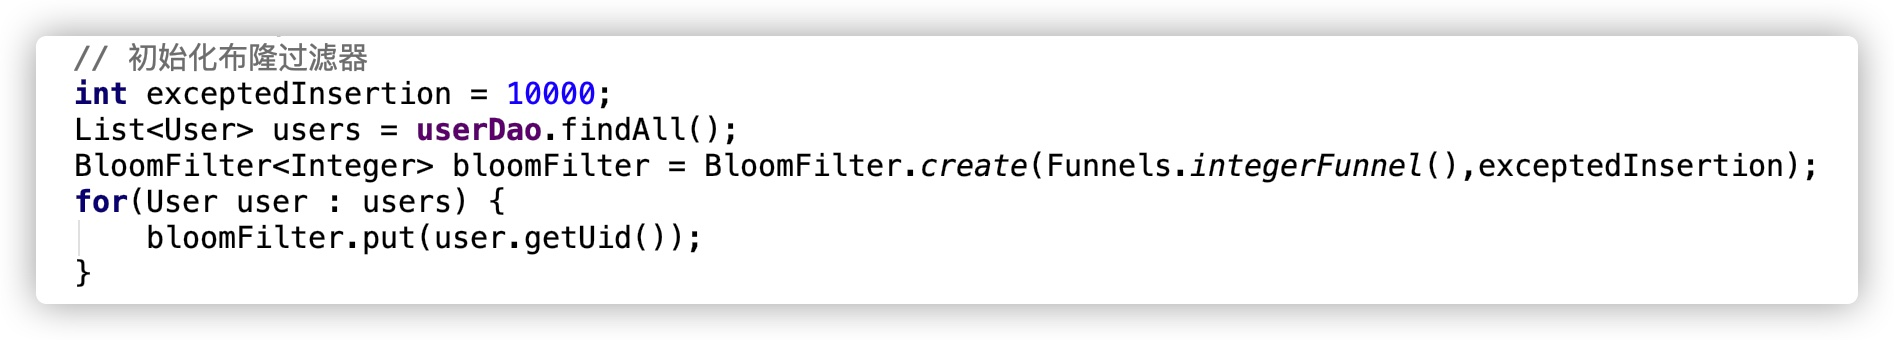
\includegraphics[width=0.8\textwidth]{9_6.jpg}
    \caption{初始化布隆过滤器}
\end{figure}

\paragraph{}在业务层模拟数据查询,查询次数为10万次,每次查询先经过布隆过滤器,如果布隆过滤器显示不存在,则直接过滤查询,如果显示存在,则返回redis中的数据,如果redis中查询不到,则继续到数据库查询数据。
\begin{figure}[!htb]
    \centering
    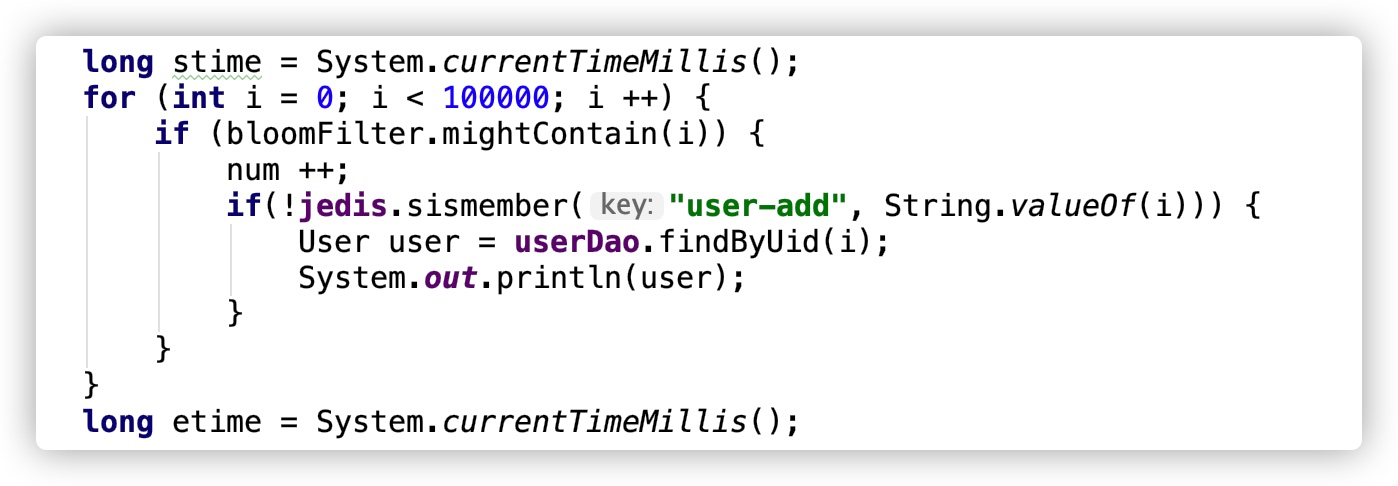
\includegraphics[width=0.7\textwidth]{9_7.jpg}
    \caption{业务查询,时间统计}
\end{figure}

\subsection{实验结果}
\paragraph{}经过与不使用布隆过滤器的情况进行对比,使用同样的业务查询次数(10万次),其耗时对比如下:
\begin{figure}[!htb]
    \centering
    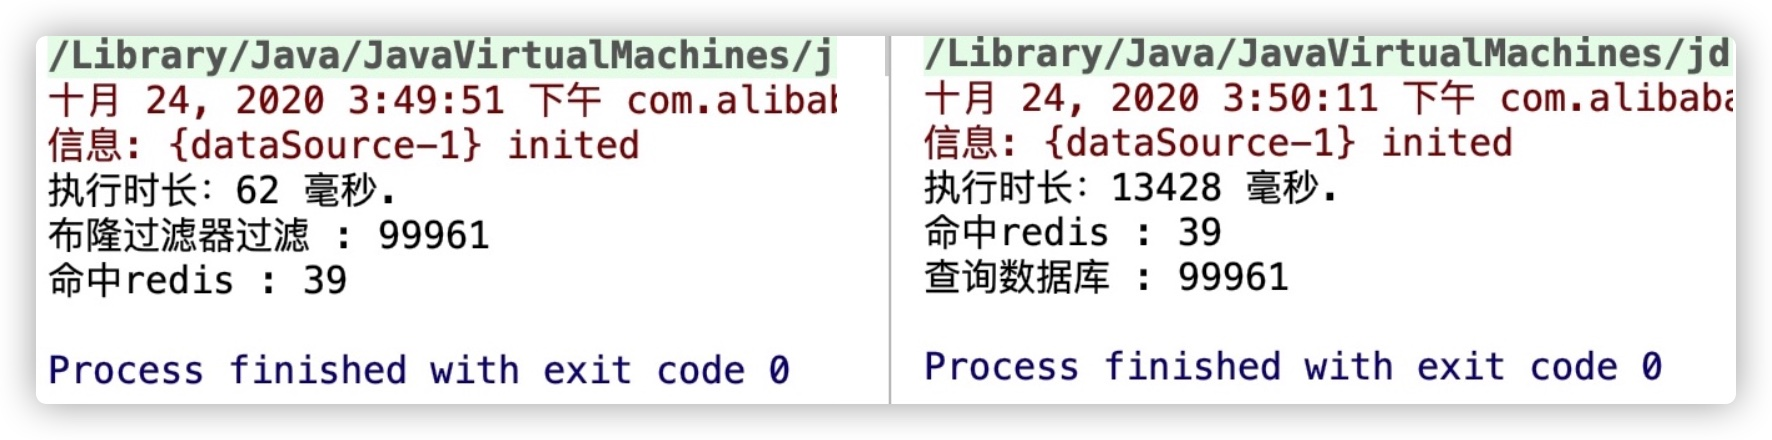
\includegraphics[width=0.7\textwidth]{11.jpg}
    \caption{使用布隆过滤器前后对比}
\end{figure}
\paragraph{}上图可以看出使用布隆过滤器和不使用过滤器的效果差距明显,耗时相差200倍。由于不使用布隆过滤器,无效查询(不存在值的查询)会避开redis,直接查询数据库,由于磁盘I/O的速度远远小于内存的计算速度,所以耗时相差非常明显,在查询次数继续增加且多线程访问的情况下,会使得MySql直接服务崩溃。
\section{总结}
\paragraph{}本文论述了redis作为缓存数据库的优势与使用场景,剖析了在使用Redis作为缓存服务器时所存在的一个缓存穿透的问题,讨论了两种缓存穿透解决方案及其优劣势,然后对布隆过滤器的原理进行了解析,最终使用布隆过滤器整合Redis和数据库进行缓存穿透的实验的设计,得出了使用布隆过滤器能极大的提升服务器查询的性能的结论,缓解Redis缓存数据库和磁盘数据库的压力,避免服务器因为缓存穿透这个漏洞而让黑客有机可乘,影响正常的业务。但是布隆过滤器还是有他的缺陷,比如误算率是其中之一,另外一般情况下不能从布隆过滤器中删除元素。目前也有很多更好的办法可以克服布隆过滤器的缺陷,比如设计一个带计数器的布隆过滤器,以空间换时间,给每一位增加计数位。所以此问题还有很多可以值得探讨的方向,本文只是浅尝辄止,还需要更深入的研究与发现,才能设计出更优更好的解决方案!
\end{document}

